\documentclass[a4paper,11pt]{article}
\usepackage[utf8]{inputenc}
\usepackage[T1]{fontenc}
\usepackage[brazilian]{babel}
\usepackage{lmodern}
\usepackage[margin=2.3cm]{geometry}
\usepackage{amsmath,amssymb}
\usepackage{booktabs}
\usepackage{graphicx}
\graphicspath{{../figures/}}
\usepackage[font=small,labelfont=bf,skip=4pt]{caption}
\usepackage{xcolor}
\usepackage{tikz}
\usetikzlibrary{positioning,calc,fit,backgrounds,arrows.meta}
\usepackage{pgfplots}
\pgfplotsset{compat=1.16}
\usepackage{enumitem}
\setlist{itemsep=2pt,topsep=3pt}
\usepackage{float}
\usepackage{microtype}
\usepackage{titlesec}
\titleformat{\section}{\normalfont\Large\bfseries}{\thesection}{0.6em}{}
\titleformat{\subsection}{\normalfont\large\bfseries}{\thesubsection}{0.6em}{}
\usepackage[colorlinks=true,linkcolor=blue!40!black,citecolor=blue!40!black,urlcolor=blue!50!black]{hyperref}

\definecolor{azul}{RGB}{37,99,235}
\definecolor{laranja}{RGB}{217,119,6}
\definecolor{verde}{RGB}{22,128,61}
\definecolor{cinza}{RGB}{110,110,110}

\newcommand{\caixa}[2]{\begin{center}\fcolorbox{#1}{#1!6}{\begin{minipage}{0.94\textwidth}\small #2\end{minipage}}\end{center}}

\title{\vspace{-1.2cm}\textbf{How Many Voices Does It Take to Clone One?}\\[4pt]
\large Dados, resultados e proposta de pesquisa: lei de escala da clonagem de voz\\ \textit{zero-shot} e uma arquitetura que separa conteúdo e voz}
\author{Richard Viana\\[2pt]\small Projeto derivado do trabalho final de Machine Learning II --- IMPA Tech}
\date{\small Documento de trabalho --- novembro de 2026}

\begin{document}
\maketitle

\begin{abstract}
\noindent Este documento reúne tudo o que o projeto tem até agora, para que alguém de fora entenda o trabalho só por ele. Partimos de um sistema de síntese de fala com estilo copiado de um áudio de referência (Tacotron~2 + VAE) e o usamos como bancada barata para uma pergunta de dados: \emph{quantos locutores, e quantas frases por locutor, um modelo precisa ver no treino para copiar a voz de alguém que nunca ouviu?} Em 33 treinos controlados (grade de $N$ locutores $\times$ $K$ frases, até $N=200$), as vozes treinadas dependem de $K$ e as vozes novas dependem de $N$. Medida em 38 vozes nunca ouvidas, a cópia sobe de 57\% para 70\% e 79\% com 8, 32 e 128 locutores, sem custo de inteligibilidade; com só três pontos e uma semente, a forma dessa curva (o expoente) ainda não é identificável. Cinco tentativas de contornar a falta de locutores falharam (troca de referência, perda contrastiva, vetor de locutor pré-treinado, pseudo-locutores por mudança de velocidade, média de referências), e a análise por voz indica que o gargalo é o \emph{decodificador} conseguir renderizar a voz, não o codificador descrevê-la. Uma revisão crítica mostra que parte da dificuldade medida vem da própria régua (a cópia é medida contra a voz padrão) e propõe um modelo de ``cobertura + atração pela voz padrão''. A partir disso propomos (i) uma lei de escala com regimes paramétrico e não paramétrico e (ii) uma arquitetura em duas etapas em que a voz é aprendida com áudio \emph{sem transcrição}, com previsões falseáveis a testar numa GPU dedicada. A aplicação-alvo é a dublagem para línguas com poucos locutores gravados, como o português.
\end{abstract}

\tableofcontents
\newpage

%=====================================================================
\section{Motivação e pergunta}

A meta de longo prazo é \textbf{dublar filmes}: dado o texto traduzido e o áudio do ator original, gerar a fala na língua de destino com a voz e o estilo do ator. Isso exige clonagem de voz \emph{zero-shot}: o modelo recebe um trecho curto de uma voz que nunca ouviu e fala um texto novo com ela.

Os sistemas atuais de clonagem treinam com dezenas de milhares de horas e milhares de locutores. Línguas como o português têm corpora transcritos com poucas dezenas de locutores. A pergunta que guia o projeto é, portanto, de dados:

\caixa{azul}{\textbf{Pergunta central.} Quantos locutores ($N$) e quantas frases por locutor ($K$) o treino precisa para que o modelo copie vozes novas sem perder inteligibilidade? Qual é a forma funcional dessa dependência, e o que limita a cópia: o codificador descrever a voz nova ou o decodificador conseguir reproduzi-la?}

O modelo usado (Tacotron~2 + VAE) é antigo e não é o que se usaria num produto hoje (Seção~\ref{sec:limites}). Ele foi escolhido como \emph{bancada}: permite dezenas de treinos controlados com orçamento de estudante. O que se pretende levar adiante é a pergunta, o protocolo e a teoria, a serem confirmados numa arquitetura atual.

%=====================================================================
\section{O que o projeto já tem}

\begin{enumerate}
\item \textbf{Um sistema de síntese em português com estilo copiado}, treinado em etapas (inglês $\rightarrow$ português $\rightarrow$ emoção) a partir do Tacotron~2 pré-treinado da NVIDIA. Palavras erradas (WER, via Whisper): 2,2\% em inglês, 10,5\% em português; o tom da fala gerada acompanha o da referência (correlação 0,97 em 10 referências de emoção).
\item \textbf{Uma correção documentada}: a versão anterior do trabalho tinha um resultado central (``atenção espectral interpretável'') que vinha de um erro de código (um \texttt{view} sem transpor tempo e frequência). O erro foi corrigido e o resultado retirado.
\item \textbf{O experimento de cobertura} ($N \times K$): 33 treinos, avaliação automática de inteligibilidade e de cópia de voz, incluindo uma avaliação em 38 vozes nunca ouvidas.
\item \textbf{Uma nota teórica} com uma lei de escala em dois níveis, previsões registradas \emph{antes} de cada experimento e o resultado de cada uma (acertos e erros).
\item \textbf{Código reprodutível} (treino, avaliação, ajuste das leis, análise por voz), resultados por amostra versionados no repositório e cópia no \textit{bucket} do projeto.
\end{enumerate}

%=====================================================================
\section{Arquitetura atual}

\begin{figure}[H]
\centering
\resizebox{\textwidth}{!}{%
\begin{tikzpicture}[
  box/.style={rectangle, draw=black!30, rounded corners=5pt, fill=black!3, minimum height=1.15cm, align=center, font=\small, inner xsep=5pt},
  hl/.style={box, draw=azul, line width=1pt, fill=azul!5},
  op/.style={box, draw=laranja, line width=1pt, fill=laranja!6, dashed},
  frozen/.style={box, fill=black!8},
  arr/.style={-{Stealth[length=2.2mm]}, semithick, draw=black!55}
]
\node[box] (txt) at (0,0) {Texto\\{\scriptsize caracteres / fonemas}};
\node[box] (enc) at (3.2,0) {Encoder de texto\\{\scriptsize Conv1d + BiLSTM}};
\node[circle, draw=azul, thick, fill=white, inner sep=1.5pt] (soma) at (5.5,0) {$+$};
\node[box] (att) at (7.6,0) {Atenção\\{\scriptsize por localização}};
\node[box] (dec) at (10.4,0) {Decoder\\{\scriptsize autorregressivo}};
\node[frozen] (voc) at (13.3,0) {HiFi-GAN\\{\scriptsize congelado}};
\node[box] (wav) at (15.6,0) {Áudio};
\node[box] (ref) at (0.4,2.3) {Mel de referência\\{\scriptsize $80\times T$}};
\node[hl] (vae) at (5.5,2.3) {Reference encoder + VAE\\{\scriptsize 6 Conv2d + GRU $\rightarrow (\mu,\sigma)$, $z\in\mathbb{R}^{32}$}};
\node[op] (spk) at (11.0,2.3) {Vetor de locutor ECAPA\\{\scriptsize congelado (só variantes \texttt{-spk})}};
\draw[arr] (txt) -- (enc); \draw[arr] (enc) -- (soma); \draw[arr] (soma) -- (att);
\draw[arr] (att) -- (dec); \draw[arr] (dec) -- (voc); \draw[arr] (voc) -- (wav);
\draw[arr] (ref) -- (vae);
\draw[arr] (vae.south) -- node[left, font=\scriptsize] {estilo $e$ $\times$ força} (soma.north);
\draw[arr, dashed, draw=laranja] (spk.south) |- (6.3,1.05) -- (soma.north east);
\end{tikzpicture}}
\caption{Tacotron~2 + VAE. O vetor de estilo $e$ (projeção de $z$), multiplicado por um fator de força (1,0 = estilo inteiro), é somado a cada posição da memória do encoder. A entrada tracejada (vetor de locutor ECAPA pré-treinado) só existe nas variantes \texttt{-spk}/\texttt{-spkdrop}. 28,9\,M de parâmetros.}
\label{fig:arq}
\end{figure}

\paragraph{Perda.} $\mathcal{L} = \mathcal{L}_{\text{mel}} + \mathcal{L}_{\text{gate}} + \beta\,\mathcal{L}_{\text{KL}} + \lambda\,\mathcal{L}_{\text{GA}}$: erro quadrático do mel, entropia cruzada do sinal de parada, divergência KL do VAE com peso crescente (cerca de 0,024 ao fim do treino de cobertura) e atenção guiada ($\lambda = 2$, $\sigma=0{,}4$).

%=====================================================================
\section{Dados e ferramentas}

\begin{table}[H]
\centering\small
\begin{tabular}{@{}p{3.6cm}p{4.4cm}p{7.6cm}@{}}
\toprule
Conjunto & Conteúdo & Uso no projeto\\
\midrule
LJSpeech & 1 locutora, inglês, 23,7\,h & Voz padrão: 2.000 frases em todo treino de cobertura\\
LibriTTS \textit{train-clean-100} & 247 locutores, inglês, $\approx$54\,h & Os $N$ locutores do treino (até 200 usados)\\
LibriTTS \textit{test-clean} & 39 locutores, inglês & 38 vozes externas da avaliação larga\\
TTS-Portuguese Corpus & 1 locutor, português, 3,8\,h & Sistema em português\\
VERBO & 12 locutores, 7 emoções, 1.167 falas & Etapa de emoção\\
\midrule
HiFi-GAN universal & vocoder pré-treinado & Mel $\rightarrow$ áudio (congelado)\\
Whisper (\textit{faster-whisper}) & reconhecimento de fala & Inteligibilidade (WER)\\
Resemblyzer & codificador de locutor & Medida de cópia de voz\\
ECAPA-TDNN & codificador de locutor & Variantes \texttt{-spk} (entrada do modelo)\\
\bottomrule
\end{tabular}
\caption{Dados e modelos auxiliares. Para medir cópia usa-se um codificador (Resemblyzer) diferente do que entra no modelo (ECAPA), para não avaliar com a mesma régua que treina.}
\end{table}

\paragraph{Computação.} Todos os treinos de cobertura rodaram em GPUs alugadas (Colab: L4 e A100), cerca de 2,5\,h por treino de 2.500 passos. Não há checkpoints guardados dos treinos de cobertura, só os resultados por amostra e os latentes de cerca de 1.500 frases por treino.

%=====================================================================
\section{O experimento de cobertura}

\subsection{Desenho}

\begin{figure}[H]
\centering
\resizebox{0.95\textwidth}{!}{%
\begin{tikzpicture}[
  box/.style={rectangle, draw=black!30, rounded corners=5pt, fill=black!3, minimum height=1.1cm, align=center, font=\small, inner xsep=7pt},
  hl/.style={box, draw=azul, line width=1pt, fill=azul!5},
  arr/.style={-{Stealth[length=2.4mm]}, semithick, draw=black!55}
]
\node[box] (lj) at (0,1.1) {LJSpeech\\{\scriptsize 2.000 frases, voz padrão}};
\node[box] (lt) at (0,-1.1) {LibriTTS\\{\scriptsize $N$ locutores $\times$ $K$ frases}};
\node[hl] (tr) at (4.6,0) {Ajuste fino\\{\scriptsize do modelo em inglês, 2.500 passos}};
\node[box] (m) at (8.6,0) {Modelo\\$(N,K,\text{semente})$};
\node[box, align=left] (ev) at (13.6,0) {Síntese de 25 frases novas com referências:\\
{\scriptsize $\bullet$ 8 vozes treinadas (frases fora do treino)}\\
{\scriptsize $\bullet$ 4 vozes novas fixas (LibriTTS, nunca treinadas)}\\
{\scriptsize $\bullet$ 4 ou 38 vozes externas (test-clean)}};
\node[box, align=left] (me) at (13.6,-2.5) {{\scriptsize WER: Whisper transcreve, compara com o texto}\\{\scriptsize Copiada: $\mathrm{sim}(\hat x, \text{ref}) > \mathrm{sim}(\hat x, \text{voz padrão})$}};
\draw[arr] (lj) -- (tr); \draw[arr] (lt) -- (tr); \draw[arr] (tr) -- (m); \draw[arr] (m) -- (ev); \draw[arr] (ev) -- (me);
\end{tikzpicture}}
\caption{Protocolo. As seleções são aninhadas (os locutores de $N=8$ estão dentro de $N=32$, as frases de $K=8$ dentro de $K=32$), de modo que treinos diferem só no que foi acrescentado.}
\end{figure}

\paragraph{Métricas.} \emph{WER}: palavras erradas na transcrição automática. \emph{Voz copiada}: fração das amostras cujo áudio está mais perto (cosseno do Resemblyzer) da referência do que da voz padrão. É uma medida binária e relativa à voz padrão, o que tem consequências (Seção~\ref{sec:porvoz}). Variantes medem também a similaridade com a média de até 20 frases do locutor da referência (\texttt{sim\_spk}).

\subsection{Grade $N \times K$}

\begin{table}[H]
\centering\small
\begin{tabular}{@{}rrcccc@{}}
\toprule
$N$ & $K$ & WER treinadas & WER novas & Copiada: treinadas & Copiada: novas\\
\midrule
2 & 128 & 13\% / 11\% & 8\% / 5\% & 70\% / 74\% & 4\% / 2\%\\
8 & 8 & 21\% / 26\% & 14\% / 24\% & 45\% / 44\% & 26\% / 39\%\\
8 & 32 & 17\% & 14\% & 74\% & 47\%\\
8 & 128 & 11\% / 10\% & 8\% / 9\% & 91\% / 88\% & 51\% / 37\%\\
32 & 8 & 17\% / 17\% & 13\% / 9\% & 58\% / 51\% & 47\% / 47\%\\
32 & 32 & 13\% & 8\% & 80\% & 52\%\\
32 & 128 & 12\% / 10\% & 5\% / 5\% & 86\% / 86\% & 61\% / 57\%\\
128 & 8 & 12\% & 8\% & 52\% & 55\%\\
128 & 32 & 12\% / 13\% & 8\% / 8\% & 76\% / 66\% & 74\% / 56\%\\
200 & 32 & 12\% & 7\% & 66\% & 64\%\\
\bottomrule
\end{tabular}
\caption{Passo 2.500, estilo inteiro. ``Novas'' = as 4 vozes fixas nunca treinadas (25 frases cada). Dois números = duas sementes. As 4 vozes dão uma medida ruidosa: entre sementes a diferença chega a 18 pontos.}
\label{tab:grade}
\end{table}

\begin{figure}[H]
\centering
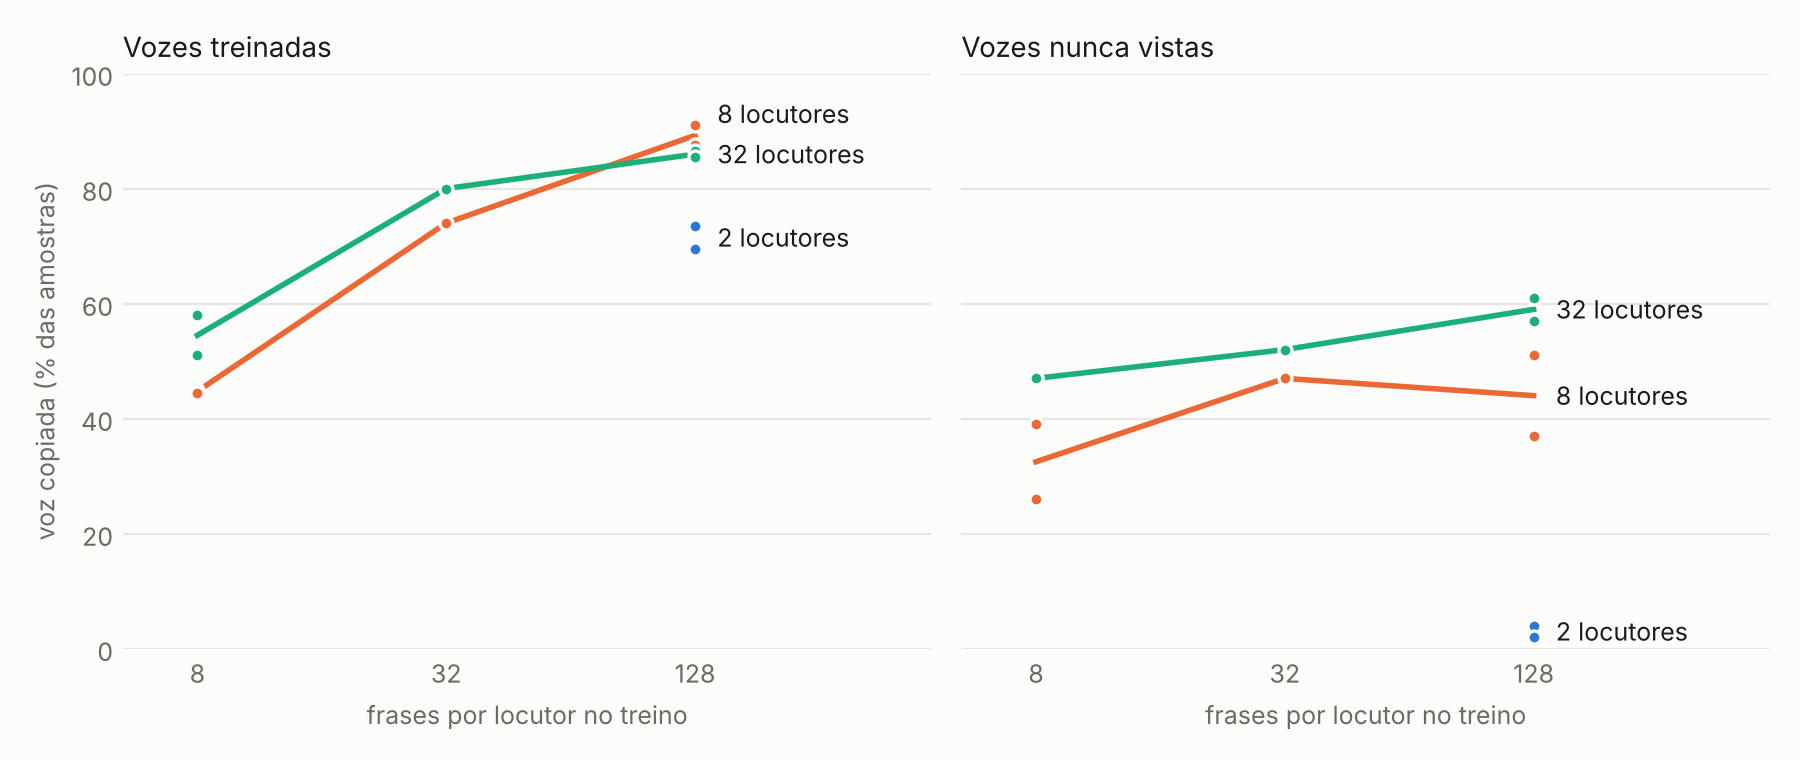
\includegraphics[width=0.82\textwidth]{fig_cobertura}
\caption{Voz copiada em função das frases por locutor ($K$) e do número de locutores ($N$), grade original ($N\le32$).}
\end{figure}

\caixa{verde}{\textbf{Resultado 1 (dois níveis).} As vozes treinadas dependem de $K$: com 8 locutores, a cópia vai de 45\% ($K=8$) a 74\% (32) e 90\% (128). As vozes novas dependem de $N$: com $K=128$, de 3\% ($N=2$) a 44\% (8) e 59\% (32). Muitos locutores compensam poucas frases: $32\times 8$ (256 frases) copia vozes novas tanto quanto $8 \times 128$ (1.024 frases).}

\subsection{Avaliação larga: 38 vozes nunca ouvidas}

Como 4 vozes dão uma medida ruidosa, três treinos com $K=32$ foram avaliados em 38 locutores do LibriTTS \textit{test-clean} (950 amostras por treino). Os intervalos de 95\% vêm de reamostrar os locutores (10.000 vezes), e as diferenças entre treinos são pareadas nos mesmos locutores.

\begin{figure}[H]
\centering
\begin{minipage}{0.48\textwidth}
\centering
\begin{tikzpicture}
\begin{axis}[width=\linewidth, height=6cm, xmode=log, log basis x=2, xtick={8,32,128}, xticklabels={8,32,128},
  xlabel={locutores no treino ($N$)}, ylabel={vozes externas copiadas (\%)}, ymin=35, ymax=95, grid=major, grid style={black!12},
  xmin=5, xmax=200, legend style={font=\scriptsize, at={(0.03,0.97)}, anchor=north west}]
\addplot+[azul, mark=*, thick, error bars/.cd, y dir=both, y explicit] coordinates {(8,57) +- (0,13.5) (32,70) +- (0,11.5) (128,79) +- (0,10.5)};
\addlegendentry{medido (IC 95\%)}
\addplot[laranja, dashed, thick, domain=5:200, samples=40] {100*(1-0.74*x^(-0.26))};
\addlegendentry{$1-c\,N^{-\alpha}$ (só descreve)}
\end{axis}
\end{tikzpicture}
\end{minipage}\hfill
\begin{minipage}{0.48\textwidth}
\small
\begin{tabular}{@{}lccc@{}}
\toprule
Treino & Copiadas & WER & Por locutor\\
 & (IC 95\%) & & $R=1 \rightarrow 4$\\
\midrule
$8\times32$ & 57\% (43--70) & 13\% & 66\% $\rightarrow$ 64\%\\
$32\times32$ & 70\% (58--81) & 12\% & 81\% $\rightarrow$ 79\%\\
$128\times32$ & 79\% (68--89) & 12\% & 88\% $\rightarrow$ 84\%\\
\bottomrule
\end{tabular}\\[6pt]
Ganho pareado: 13 pontos de 8 para 32 (IC 4--23); 9 pontos de 32 para 128 (IC 1,5--17).
\end{minipage}
\caption{Cópia de voz em 38 vozes nunca ouvidas. A curva tracejada é uma potência passando pelos três pontos ($\alpha=0{,}26$); com dois parâmetros, três pontos e uma semente, ela descreve e não testa nada: qualquer $\alpha$ entre cerca de 0,06 e 0,53 seria compatível (Seção~\ref{sec:revisao}). ``$R=4$'': código de estilo tirado da média de 4 frases do locutor.}
\label{fig:larga}
\end{figure}

\caixa{verde}{\textbf{Resultado 2 (mais locutores continuam rendendo).} De 8 para 32 e de 32 para 128 locutores a cópia de vozes novas sobe 13 e 9 pontos, com WER constante (12--13\%); o ganho de 32 para 128 é real (IC não inclui zero). A impressão anterior, vinda das 4 vozes, de que acima de 128 locutores não havia ganho era ruído de medida. O que \emph{não} está estabelecido é a forma da curva: o expoente e qualquer extrapolação para milhares de locutores.}

\subsection{Tentativas de contornar a falta de locutores (todas negativas)}

\begin{table}[H]
\centering\small
\begin{tabular}{@{}p{4.1cm}p{5.1cm}p{5.6cm}@{}}
\toprule
Ideia & Hipótese testada & Resultado\\
\midrule
Troca de referência (\texttt{-swap}) e perda contrastiva (\texttt{-contrast}) & O código de estilo carrega o conteúdo da frase & Nada muda além da variação entre sementes (ex.: $8\times128$: novas 51\% $\rightarrow$ 38--39\%)\\
Vetor de locutor ECAPA congelado (\texttt{-spk}) & Um codificador treinado em milhares de vozes descreve vozes novas & O modelo ignora a entrada: sem o VAE, 0\% de cópia\\
ECAPA + \textit{dropout} do VAE (\texttt{-spkdrop}) & Forçar a voz a passar pelo vetor & Com 8 locutores o vetor sozinho copia 71\% das treinadas e 5\% das novas: decora. Com 32 locutores, vetor + VAE = treino normal\\
Pseudo-locutores por mudança de velocidade (\texttt{-aug}) & Vozes alteradas contam como locutores novos & Previsto 31\% (não contam) ou 50\% (contam); medido 28\%. Idem com $K=128$: 42\% (previsto 44\% / 55\%). Não contam\\
Média de 4 ou 16 referências & O erro vem do ruído de uma referência só & Ajuda nas 4 vozes da grade, mas não nas 38 externas (cai 2 a 4 pontos); só reduz o WER em 1 a 3 pontos\\
\bottomrule
\end{tabular}
\caption{Variantes testadas, com previsões registradas antes nos casos indicados.}
\label{tab:neg}
\end{table}

\caixa{laranja}{\textbf{Resultado 3 (o que não resolve).} Nem um codificador melhor, nem referências melhores, nem perdas no latente, nem vozes artificiais simples substituem o decodificador ter ouvido muitas vozes reais.}

\subsection{Quais vozes falham, e por quê}
\label{sec:porvoz}

Correlações de postos sobre os 38 locutores externos (\texttt{scripts/coverage/voice\_hardness.py}):
\begin{itemize}
\item \textbf{A dificuldade é da voz:} a taxa de cópia por locutor se correlaciona 0,75 entre $N=8$ e 32, 0,74 entre 32 e 128, 0,59 entre 8 e 128. Em todos os treinos há vozes com 0\% e com 100\%: a cópia é quase tudo-ou-nada por voz.
\item \textbf{Vozes agudas falham mais} ($-0{,}53$, $-0{,}52$, $-0{,}37$ entre cópia e F0 da referência). A voz padrão é feminina; a cópia sobe com a distância (no latente) até a voz padrão (0,47; 0,58; 0,53). Parte da falha é atração pela voz padrão, e parte pode ser artefato da medida relativa.
\item \textbf{A distância à voz treinada mais próxima prevê a falha com poucos locutores e deixa de prever com muitos:} $-0{,}33$ ($N=8$), $-0{,}40$ ($N=32$), $+0{,}13$ ($N=128$).
\end{itemize}

\subsection{Informação no latente de estilo}

\begin{table}[H]
\centering\small
\begin{tabular}{@{}lccc@{}}
\toprule
Treino & Bits por frase (KL) & Bits sobre o locutor (aprox.) & $\log_2$(nº de locutores)\\
\midrule
$2\times128$ & 64 & 5 & 1,6\\
$8\times32$ & 67 & 10 & 3,2\\
$32\times32$ & 72 & 16 & 5,0\\
$128\times32$ & 73 & 19 & 6,9\\
$200\times32$ & 72 & 20 & 7,4\\
\bottomrule
\end{tabular}
\caption{O KL por frase é uma cota superior da informação que passa pelo latente (as 32 dimensões estão ativas em todos os treinos). ``Bits sobre o locutor'' usa uma aproximação gaussiana (covariância total sobre covariância dentro do locutor); a revisão (Seção~\ref{sec:revisao}) mostra que o viés é pequeno, mas que o número mede um vetor de voz contínuo, não a identidade entre os $N$ locutores. Cerca de 80\% da variância do latente é entre locutores, e a distância do código à voz padrão tem correlação 0,83 com a cópia.}
\label{tab:info}
\end{table}

O canal de estilo carrega 65--73 bits por frase (KL), mas a maior parte paga o posterior estreito; a informação estimada sobre a voz fica perto de 17 bits e não cresce de $N=32$ a 200. O latente não está saturado: o limite não é capacidade, é quantas vozes o decodificador ouviu.

%=====================================================================
\section{Teoria}

\subsection{Lei em dois níveis}

Locutores são sorteados de uma população; frases são sorteadas dentro de cada locutor. Num modelo hierárquico (efeitos aleatórios) de dimensão finita, o erro numa voz treinada tem um termo que cai com $K$, e o erro numa voz nova tem um termo que cai com $N$ e outro com $NK$:
\begin{align*}
\text{treinadas não copiadas} &\approx a' + \frac{C}{K} + \frac{A'}{N}, &
\text{novas não copiadas} &\approx a + \frac{A}{N} + \frac{B}{NK}.
\end{align*}
Ajuste em 16 treinos: $a'=0{,}14$, $C=2{,}87$, $A'=0{,}22$ (RMSE 0,057); $a=0{,}39$, $A=1{,}08$, $B=10{,}3$ (RMSE 0,060). É a forma da decomposição de variância em amostragem de dois estágios e das cotas de meta-aprendizado com tarefas gaussianas.

\subsection{Dois regimes e o expoente}

A forma acima prevê queda em $1/N$ até um piso $a\approx0{,}39$. A alternativa $a + A/\sqrt N + C/\sqrt K$ ajusta igualmente bem (RMSE 0,056, piso 0,19). A avaliação larga (Fig.~\ref{fig:larga}) mostra não copiadas 43\% $\rightarrow$ 30\% $\rightarrow$ 21\%, que uma potência $N^{-0{,}26}$ atravessa exatamente. Pelo critério registrado antes do experimento a razão entre os ganhos (0,7) favorecia a lei com raízes, mas a revisão estatística (Seção~\ref{sec:revisao}) mostra que nenhuma das leis se distingue das outras com estes dados.

\caixa{azul}{\textbf{Interpretação proposta.} Há dois regimes:
\begin{itemize}[leftmargin=12pt]
\item \emph{paramétrico}: a voz vive numa família de baixa dimensão $k$ que o decodificador aprende como regra; o erro cai como $k/N$ (rápido);
\item \emph{não paramétrico} (``cobertura''): o decodificador só reproduz vozes perto das que ouviu; o erro é governado pela distância à voz treinada mais próxima, que cai como $N^{-1/d}$ num espaço de vozes de dimensão intrínseca $d$ (lento).
\end{itemize}
A dimensão do espaço de vozes medida no latente é de 7 a 10 (Seção~\ref{sec:revisao}), o que descarta a versão mais simples (falha proporcional à distância, que pediria $d\approx4$ para $\alpha=0{,}26$); falha proporcional ao quadrado da distância pede $d\approx7{,}7$ e é compatível, sem ser um teste. A análise por voz (distância à voz mais próxima prevê a falha com $N$ pequeno) e o fracasso de codificadores e referências melhores apontam para o regime de cobertura.}

\subsection{Consequências e previsões da teoria}
\begin{itemize}
\item Se o regime é de cobertura, \textbf{melhorar o codificador não muda o expoente}; mudar o que o decodificador ouviu, sim (consistente com a Tabela~\ref{tab:neg}).
\item Uma arquitetura que force a dependência da voz a uma família de baixa dimensão deveria trocar a queda lenta pela queda em $1/N$, ao preço de um piso se o espaço real de vozes tiver mais dimensões que o módulo.
\item As extrapolações para milhares de locutores que constavam da versão anterior deste documento foram retiradas: não têm apoio estatístico.
\item O latente de 32 dimensões está superdimensionado para a voz: 8 a 10 dimensões deveriam bastar para a cópia (previsão do ``modelo mínimo'').
\end{itemize}

\subsection{O que já existe na literatura}
Um levantamento (cerca de 35 buscas e 5 artigos lidos na íntegra) não encontrou lei explícita de cópia de voz em função de $N$ e $K$. O fato qualitativo ``são precisos milhares de locutores'' aparece desde \cite{jia2018}, cuja tabela de codificador de locutor dá um expoente aparente de 0,21--0,25 (conta nossa, com fatores misturados). O análogo em verificação de locutor (poucos locutores vs.\ muitas sessões) está em \cite{tinyvox}. As formas $1/N + 1/(NK)$ e $1/\sqrt N + 1/\sqrt K$ vêm de meta-aprendizado \cite{du2021,maurer2016}; expoentes ligados à dimensão dos dados, de \cite{sharma2020,bahri2021}. A capacidade do latente de estilo em bits já foi usada em \cite{capacitron}. O que parece novo: a lei fatorial $N\times K$ para clonagem, a ligação do expoente com a dimensão do espaço de \emph{locutores} (as amostras são grupos, não frases) e a decomposição dos bits do latente em voz e resto. A busca não cobriu o ISCA Archive nem o IEEE Xplore.

%=====================================================================
\section{Revisão crítica (três análises sem treino novo)}
\label{sec:revisao}

Três análises independentes, só com CPU sobre os dados salvos, revisaram as afirmações acima (relatórios completos em \texttt{reports/teoria/}). O que mudou:

\paragraph{A régua.} Com vetores de locutor normalizados, a margem medida tem uma forma exata:
\[
m = \mathrm{sim}_{\text{ref}} - \mathrm{sim}_{\text{padrão}} = \left(\tfrac12 - \rho\right)\lVert e_{\text{ref}} - e_0\rVert^2,
\]
em que $\rho$ é quanto a saída é puxada para a voz padrão ao longo do eixo referência--padrão. A voz conta como copiada se e só se $\rho<\tfrac12$, e o tamanho da margem é proporcional a $\lVert e_{\text{ref}}-e_0\rVert^2$: vozes parecidas com a voz padrão têm margens minúsculas e mudam de lado por ruído. Pitch e semelhança com a voz padrão explicam 28--59\% da dificuldade das vozes na medida binária e só 2--9\% na semelhança direta com a referência. Parte da ``dificuldade das vozes agudas'' é, portanto, da régua.

\paragraph{O expoente.} A potência $N^{-0{,}26}$ é exatamente o que dois parâmetros fazem passar por três pontos de uma semente. Numa simulação com a variância medida, esse desenho recupera expoentes entre 0,06 e 0,53 quando o verdadeiro é 0,26, e escolhe a lei certa entre 16\% e 62\% das vezes. Com medidas que não usam a voz padrão o expoente aparente sobe para 0,41--0,55. Na grade de 4 vozes, a lei com raízes só ganha por causa dos treinos com $N=2$; sem eles, as quatro leis testadas empatam.

\paragraph{O que se mantém.} Vozes treinadas seguem só $K$ (colapso em $K^{0{,}46}$, efeito de $N$ igual a zero $\pm 0{,}07$). A cópia é quase tudo-ou-nada por voz (correlação intraclasse 0,83--0,94; dois terços das 38 vozes ficam abaixo de 10\% ou acima de 90\%). A variação vem da voz de referência (desvio 0,095 na margem) e não da frase (0,007); entre sementes, o desvio da fração copiada é de 7,7 pontos, dos quais cerca de 40\% é só ruído de ressíntese. A média de 4 referências não melhora a cópia nas 38 vozes ($-2{,}5$ pontos, IC $[-6{,}4; +0{,}8]$) e reduz o WER em 1,8 ponto.

\paragraph{Informação e dimensão.} Dos 64--75 bits por frase do KL, 62--70 pagam o posterior estreito; a informação gaussiana sobre a frase fica em 17--29 bits e a informação sobre a voz em cerca de 17 bits na média $\mu$, estável de $N=32$ a 200. Um classificador com validação cruzada recupera 5,1--5,3 dos 6,9 bits possíveis com 128 locutores. A voz ocupa 6--8 direções úteis (razão de participação 5,8--9,7) e a dimensão intrínseca das médias por locutor é 7--10 (TwoNN 9,7--10,6; Levina--Bickel 7,0--7,5).

\paragraph{Um modelo que reproduz os fatos.} Um suavizador que pondera as vozes treinadas pelo número de frases e compete com a voz padrão (2.000 frases) dá a regra
\[
\text{copiada} \iff K\textstyle\sum_i k(v,v_i) > M\,k(v,v_0),
\]
com $M$ o número de frases da voz padrão. Com um espectro de vozes $\lambda_j\propto 1/j$ (o latente mede expoente 1,05--1,1), esse modelo reproduz a curva, os sinais das correlações por voz e a grade ($r=0{,}97$). São cinco parâmetros escolhidos com três pontos, então isto não é um teste. O modelo também prevê que os pseudo-locutores por mudança de velocidade deveriam ter contado, e eles não contaram: é a principal tensão em aberto.

\paragraph{Previsões novas e baratas.}
\begin{itemize}
\item \textbf{Metade das frases da voz padrão equivale a dobrar $K$} para as vozes novas (consequência direta da regra acima). Custa dois treinos.
\item \textbf{Latente de 8 dimensões} não muda a cópia; com 2 dimensões, cai. A taxa pode descer a 25--30 bits por frase sem perda.
\item \textbf{$N=2.456$, $K=32$}: cerca de 9\% de vozes não copiadas sob o modelo de cobertura contra 16\% ou mais sob as leis com piso; decidir isso exige pelo menos 200 vozes de avaliação.
\item \textbf{Sem treino}: o espectro dos vetores de locutor do LibriTTS decide entre os regimes e fixa o piso de um módulo de voz de dimensão $k$.
\item \textbf{Duas etapas}: a cópia segue $N_{\text{voz}}$ se as unidades de conteúdo vazarem pouca informação de voz; um vazamento de peso 0,2 já impõe um piso de cerca de 15\% de vozes não copiadas.
\end{itemize}

%=====================================================================
\section{Limites do que temos}
\label{sec:limites}
\begin{itemize}
\item \textbf{Arquitetura antiga.} Tacotron~2 (2017) foi superado por modelos de linguagem sobre tokens de codec e por modelos de \textit{flow matching}/difusão treinados em dezenas de milhares de horas. A atenção do Tacotron é frágil e a qualidade bate num teto. O resultado só vale para a área se se repetir num modelo atual.
\item \textbf{Escala pequena.} $N\le200$, uma semente na maior parte das células, 2.500 passos. Três pontos na avaliação larga não distinguem potência de logaritmo.
\item \textbf{Uma medida.} A cópia depende de um codificador de locutor e é relativa à voz padrão, o que distorce a dificuldade das vozes parecidas com ela (Seção~\ref{sec:revisao}); não há teste de escuta nem medida de naturalidade.
\item \textbf{Sem checkpoints.} A conta de bits por parâmetro do decodificador não pode ser feita com o que foi guardado.
\end{itemize}

%=====================================================================
\section{Proposta}

\subsection{Pergunta e hipótese}

\caixa{azul}{\textbf{Pergunta.} A cópia de vozes novas depende do número de locutores no áudio \emph{transcrito} ou do número de locutores que o módulo de voz ouviu, transcrito ou não?\\[3pt]
\textbf{Hipótese.} Se a voz é aprendida por uma etapa separada, a partir de áudio sem transcrição, a cópia passa a seguir o número de locutores dessa etapa, com a mesma lei; poucos locutores transcritos bastam para o conteúdo. Para clonar bem, junte vozes, não transcrições.}

\subsection{Arquitetura proposta: conteúdo e voz separados}

\begin{figure}[H]
\centering
\resizebox{\textwidth}{!}{%
\begin{tikzpicture}[
  box/.style={rectangle, draw=black!30, rounded corners=5pt, fill=black!3, minimum height=1.15cm, align=center, font=\small, inner xsep=5pt},
  ca/.style={box, draw=azul, line width=1pt, fill=azul!5},
  cb/.style={box, draw=verde, line width=1pt, fill=verde!6},
  fz/.style={box, fill=black!8},
  arr/.style={-{Stealth[length=2.2mm]}, semithick, draw=black!55},
  tr/.style={-{Stealth[length=2.2mm]}, semithick, dashed, draw=black!45},
  lab/.style={font=\scriptsize, fill=white, inner sep=1pt}
]
\node[font=\small\bfseries, anchor=west] at (-1.2,3.4) {Inferência (dublagem)};
\node[box] (txt) at (0,0) {Texto traduzido\\{\scriptsize ex.: português}};
\node[ca] (A) at (3.6,0) {\textbf{Etapa A: conteúdo}\\{\scriptsize texto $\rightarrow$ unidades}\\{\scriptsize sem identidade de voz}};
\node[box] (u) at (7.0,0) {Unidades\\{\scriptsize $u_{1:T}$ + duração}};
\node[cb] (B) at (10.4,0) {\textbf{Etapa B: voz}\\{\scriptsize $(u_{1:T}, v) \rightarrow$ mel}};
\node[fz] (voc) at (13.4,0) {Vocoder};
\node[box] (out) at (16.0,0) {Fala dublada};
\node[box] (ator) at (6.4,2.2) {Áudio do ator original\\{\scriptsize qualquer língua}};
\node[cb] (ve) at (10.4,2.2) {Codificador de voz\\{\scriptsize código $v$ de baixa dimensão}};
\draw[arr] (txt) -- (A); \draw[arr] (A) -- (u); \draw[arr] (u) -- (B); \draw[arr] (B) -- (voc); \draw[arr] (voc) -- (out);
\draw[arr] (ator) -- (ve); \draw[arr] (ve) -- node[right, font=\scriptsize]{$v$} (B);
\draw[black!20] (-1.2,-1.65) -- (17.2,-1.65);
\node[font=\small\bfseries, anchor=west] at (-1.2,-2.0) {Treino};
\node[box, fill=azul!3, draw=azul!60] (dA) at (3.6,-3.6) {Áudio \textbf{transcrito}\\{\scriptsize poucos locutores ($N_{\text{texto}}$)}\\{\scriptsize língua de destino}};
\node[fz] (ssl) at (9.9,-3.6) {Extrator de unidades\\{\scriptsize auto-supervisionado, congelado}};
\node[box, fill=verde!3, draw=verde!60] (dB) at (15.3,-3.6) {Áudio \textbf{sem transcrição}\\{\scriptsize muitos locutores ($N_{\text{voz}}$)}\\{\scriptsize qualquer língua}};
\draw[tr] (dA.north) -- node[lab, right]{treina A} (A.south);
\draw[tr] (dB.west) -- node[lab, above]{áudio} (ssl.east);
\draw[tr] (ssl.north) -- node[lab, left]{unidades} (9.9,-0.6);
\draw[tr] (dB.north) -- (15.3,-1.2) -- node[lab, below]{alvo: o próprio áudio} (11.0,-1.2) -- (11.0,-0.6);
\end{tikzpicture}}
\caption{Proposta. A etapa A aprende o que falar e precisa de texto; a etapa B aprende a renderizar vozes e é treinada por reconstrução (unidades extraídas do próprio áudio $\rightarrow$ o mesmo áudio), sem texto. Os alvos da etapa A são as unidades extraídas do áudio transcrito. As setas tracejadas são treino; as contínuas, inferência. A lei de escala prevê que a cópia de vozes novas siga $N_{\text{voz}}$, não $N_{\text{texto}}$.}
\label{fig:proposta}
\end{figure}

A separação em etapas não é nova em si: há sistemas que geram primeiro tokens de conteúdo e depois o áudio, e trabalhos que usam fala sem transcrição para reduzir a necessidade de texto. O que esta proposta acrescenta é \textbf{medir de qual conjunto de dados vem a cópia de vozes e com que lei}, com o expoente previsto antes, e o caso de \textbf{línguas diferentes nas duas etapas}. Antes de investir, é preciso uma busca dedicada para confirmar que isso não foi feito.

\subsection{Experimentos planejados (GPU dedicada, NVIDIA RTX A4500, 20\,GB)}

\begin{table}[H]
\centering\small
\begin{tabular}{@{}p{0.6cm}p{4.6cm}p{5.4cm}p{4.2cm}@{}}
\toprule
& Experimento & Previsão registrada & O que decide\\
\midrule
E0 & Sem treino: espectro dos vetores de locutor do LibriTTS; pequeno teste de escuta nas vozes agudas & Espectro em $1/j$ (cobertura); ouvintes não confirmam a ``dificuldade'' das vozes agudas & Regime; quanto da curva é da régua\\
E0b & Metade das frases da voz padrão ($M=1.000$) contra o dobro de $K$ & Mesmo efeito nas vozes novas & O modelo de cobertura + atração\\
E1 & Repetir a varredura de $N$ (8 a 2.456, LibriTTS completo) numa arquitetura atual aberta, em configuração pequena; $N\in\{8,32,128,512,2048\}$, 3--5 sementes, 60--100 vozes de avaliação $\times$ 10 frases, métrica contínua sem voz padrão & Ganho continua até 2.048; não copiadas $\approx$9\% (cobertura) ou $\ge$16\% (piso) & Se a lei é do Tacotron ou da tarefa, e qual\\
E2 & Arquitetura em duas etapas: $N_{\text{texto}}=8$ fixo, $N_{\text{voz}}$ de 8 a 2.456 & Cópia segue $N_{\text{voz}}$ com o expoente de E1; WER segue $N_{\text{texto}}$ & A hipótese central\\
E3 & Etapa B em inglês, etapa A em português com poucos locutores & Cópia de vozes novas próxima da de E2; WER do português próximo do sistema atual (10\%) & Dublagem com poucos dados\\
E4 & Latente de voz menor (32 $\rightarrow$ 16, 8, 4, 2) e KL maior & Cópia inalterada com 8 dimensões e taxa de 25--30 bits; cai com 2 & O ``modelo mínimo''\\
\bottomrule
\end{tabular}
\caption{Plano. Cada previsão é escrita na nota teórica antes de rodar. O desenho de avaliação vem de uma simulação de poder com a variância medida: a partir de cerca de 40 vozes o gargalo é o número de sementes. Checkpoints passam a ser guardados para a análise de informação por parâmetro.}
\end{table}

\paragraph{Critério de sucesso.} A tese vale se, em E2, a cópia de vozes novas com 8 locutores transcritos e milhares de locutores sem transcrição ficar dentro do intervalo de um modelo treinado com milhares de locutores transcritos. Se E1 não reproduzir a lei numa arquitetura atual, o trabalho se reduz a um estudo sobre o Tacotron, e a proposta de arquitetura deve ser revista antes de E2.

\subsection{Produtos esperados}
\begin{enumerate}
\item \textbf{Artigo de workshop} com o que já existe: ``How Many Voices Does It Take to Clone One? A Scaling Law for Zero-Shot Voice Cloning'' (estudo controlado, lei em dois níveis, negativos, análise por voz).
\item \textbf{Artigo principal}, se E1--E3 confirmarem: ``Voices, Not Transcripts: Scaling Zero-Shot Voice Cloning with Untranscribed Speech''.
\item \textbf{Sistema de dublagem} para o português usando a etapa de voz treinada em outra língua.
\end{enumerate}

%=====================================================================
\section{Onde está cada coisa}

\begin{table}[H]
\centering\small
\begin{tabular}{@{}p{7.6cm}p{8cm}@{}}
\toprule
Caminho no repositório & Conteúdo\\
\midrule
\texttt{src/training/training-tacotron2-vae/} & Modelo e treino\\
\texttt{scripts/coverage/coverage\_manifest.py} & Montagem dos conjuntos $N\times K$ e das referências\\
\texttt{scripts/coverage/colab\_job.sh} & Treino e avaliação de uma rodada de ponta a ponta\\
\texttt{scripts/eval/synth\_check.py} & Síntese e WER (opção \texttt{--n-refs})\\
\texttt{scripts/coverage/speaker\_similarity.py} & Medida de cópia de voz\\
\texttt{scripts/coverage/fit\_law.py} & Ajuste das leis\\
\texttt{scripts/coverage/voice\_hardness.py} & Análise por voz\\
\texttt{reports/coverage/results/} & Resultados por amostra de todos os treinos\\
\texttt{reports/teoria\_cobertura.md} & Nota teórica com previsões e resultados em ordem cronológica\\
\texttt{reports/relatorio\_final.pdf} & Relatório do trabalho final de ML2\\
\bottomrule
\end{tabular}
\end{table}

Página do projeto: \url{https://rick0110.github.io/ml2_final_project}. Repositório: \url{https://github.com/rick0110/ml2_final_project}.

\begin{thebibliography}{99}\small
\bibitem{shen} J.~Shen et al. Natural TTS synthesis by conditioning WaveNet on mel spectrogram predictions (Tacotron~2). ICASSP, 2018.
\bibitem{hsu} W.-N.~Hsu et al. Hierarchical generative modeling for controllable speech synthesis. ICLR, 2019.
\bibitem{zhang} Y.-J.~Zhang et al. Learning latent representations for style control and transfer in end-to-end speech synthesis. ICASSP, 2019.
\bibitem{hifigan} J.~Kong, J.~Kim, J.~Bae. HiFi-GAN: generative adversarial networks for efficient and high fidelity speech synthesis. NeurIPS, 2020.
\bibitem{jia2018} Y.~Jia et al. Transfer learning from speaker verification to multispeaker text-to-speech synthesis. NeurIPS, 2018. arXiv:1806.04558.
\bibitem{tinyvox} Treino de reconhecimento de locutor com dados limitados (subconjuntos do VoxCeleb2). arXiv:2203.14688.
\bibitem{du2021} S.~Du et al. Few-shot learning via learning the representation, provably. ICLR, 2021. arXiv:2002.09434.
\bibitem{maurer2016} A.~Maurer, M.~Pontil, B.~Romera-Paredes. The benefit of multitask representation learning. JMLR, 2016. arXiv:1505.06279.
\bibitem{sharma2020} U.~Sharma, J.~Kaplan. A neural scaling law from the dimension of the data manifold. arXiv:2004.10802.
\bibitem{bahri2021} Y.~Bahri et al. Explaining neural scaling laws. PNAS, 2024. arXiv:2102.06701.
\bibitem{capacitron} E.~Battenberg et al. Effective use of variational embedding capacity in expressive end-to-end speech synthesis. arXiv:1906.03402.
\bibitem{libritts} H.~Zen et al. LibriTTS: a corpus derived from LibriSpeech for text-to-speech. Interspeech, 2019.
\bibitem{whisper} A.~Radford et al. Robust speech recognition via large-scale weak supervision. ICML, 2023.
\end{thebibliography}

\end{document}
